\section{Microsoft Azure}
Azure ist Microsofts Hybrid-Cloud-Plattform. Azure enthält eine stetig wachsende Anzahl an Tools, Diensten, Anwendungen und SQL- sowie NSQL-Datenbanken, die dem Nutzer über das Portal angeboten werden. Zudem bieten sie Dienste, mit welchen die Entwicklung intelligenter Anwendungen sowie die Forschung im Bereich Machine Learning ermöglicht wird. Nutzer können über Azure auf Hochleistungsgrafikprozessoren zugreifen, wodurch ihnen die Entwicklung im Bereich autonomes Fahren, Spracherkennung sowie Daten- und Videoanalyse erlaubt wird. Neben umfangreicher Prozessorleistung stellt Microsoft auch Speicherplatz zur Verfügung. Somit erlaubt Azure das Speichern und verknüpfen eigener Daten und Apps in der Cloud sowie lokal (daher Hybrid-Cloud) \cite{Sicherheit.2017b}. Über das Cloud-Computing-Konzept lassen sich IT-Infrastrukturen flexibel gestalten. Stichwörter hier sind Infrastructure-, Platform- und Application-as-a-Service. Auch Lösungen unter Einbeziehung von beliebige Entwicklungstools oder -sprachen werden dem Anwender ermöglicht \cite{Klein.2017}. \\ \\ 
Grundlage der Azure-Plattform ist ein wachsendes Netzwerk aus verteilten Rechenzentren. Somit kann eine hohe Verfügbarkeit gewährleistet werden. Die Sicherung der eigenen Anwendungen und Daten wird durch diese Hochverfügbarkeit und eine Notfallwiederherstellung gewährleistet. Durch kontinuierliche Investitionen in die neueste Infrastrukturtechnologie, bleibt Microsofts Plattform nachhaltig \cite{Klein.2017}.\\ \\
Derzeit liegt Microsoft hinter dem Marktführer Amazon, welches in Abbildung \ref{fig:statistik} illustriert wird. Auf der offiziellen Website von Azure wird die Frage gestellt ''Azure oder AWS?''. Microsoft gibt darauf eine prägnante Antwort: ''Azure ist die richtige Wahl'' \cite{Microsoft.2017}.
\begin{figure}[ht!]
	\centering
	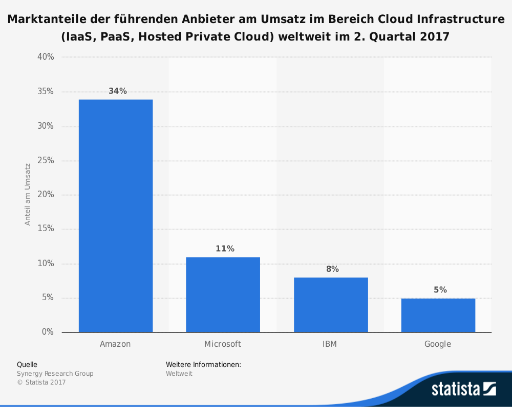
\includegraphics[width=1.0\linewidth]{images/statistik}
	\caption{Marktanteil nach Umsatz \cite{Statista.2017b}} %Generelle
	\label{fig:statistik}
\end{figure}
\\ \\Beide Plattformen haben ihre Vor- und Nachteile. Welche sich tatsächlich besser eignet, hängt von der Anforderung ab \cite{PeterTsai.2016}. Was Azure allerdings zugute kommt, ist die ergonomische Benutzeroberfläche zum Aufsetzen komplexer Systeme. Dies ist durch das Verknüpfen verschiedener Dienste möglich. Die Schritt-für-Schritt-Anleitungen, die dem Anwender zur Verfügung gestellt werden, zeigen, dass die Einrichtung entsprechender Dienste, Server und Cloud-Instanzen mit wenig Aufwand durchzuführen ist. Somit macht es den Übergang zur Cloud-basierten Infrastruktur für viele Unternehmen unbeschwerter. Vor allem das nahtlose Zusammenarbeiten der angebotenen Dienste bzw. Azure-Instanzen erlaubt es, eine robuste Infrastruktur aufzubauen. Als Exempel kann hier der IoT Hub und die sich daran anschließende Ereignisverarbeitung Azure Stream Analytics dargelegt werden \cite{PeterTsai.2016}. Eine Azure-Instanz besteht dabei aus einem virtuellen Server. Dieser wird über Hyper-V (Microsofts Hypervisor zur Visualisierung ihrer Server \cite{searchdatacenter.2017}) betrieben.\\ \\
Microsoft bietet einsatzbereite Lösungen, die vollständig vorkonfiguriert sind. So lassen sich die häufigsten Szenarien im IoT-Bereich aufsetzen, ohne dass es Cloud-Wissen oder Software-Know-How bedarf. Abbildung \ref{fig:remote_monitor} zeigt die fertige Lösung zur Überwachung der Telemetrie einiger Geräte.
\begin{figure}[ht!]
	\centering
	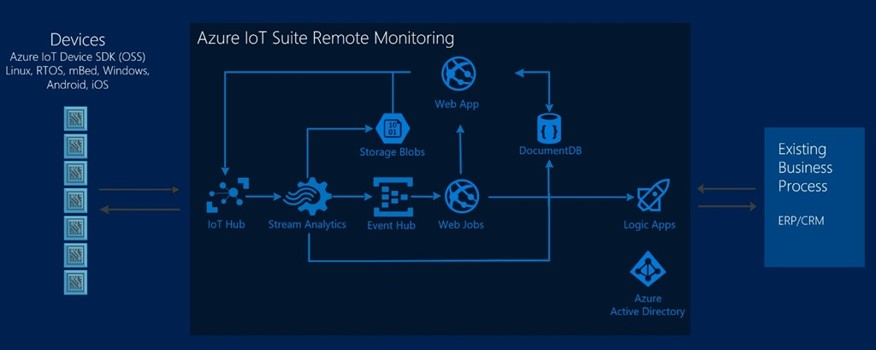
\includegraphics[width=1.0\linewidth]{images/remote_monitor}
	\caption{Fertige Remote Monitoring-Lösung \cite{Azure.2017}} %Generelle
	\label{fig:remote_monitor}
\end{figure}
\\ \\Eine weitere verfügbare Lösung wäre der vorhersagbare Wartungsbedarf. Diese Systeme sind Teil der IoT bzw. Cortana Suite. Beide Angebote bestehen aus einer Reihe von Azure-Diensten \cite{PeterTsai.2016}.  
 
